\label{sec:intro}
%Despite a lot of recent research, understanding the optimization and generalization for neural networks remain challenging problems: why can simple algorithm such as stochastic gradient descent optimize the complicated nonconvex objective, and why would the result generalize to unseen data? A common conjecture is that both problems are related to the loss landscape of neural networks. In this paper, we focus on an important aspect of the loss landscape \--- the layer-wise Hessian for neural networks along its training trajectory.

Neural network objectives are complicated and non-convex. However, in practice neural networks can be trained by simple algorithms and they perform well on test data. A common explanation is that neural network objectives have good loss landscapes for optimization and generalization. In this paper we study the structure of Hessians for neural network objectives.

Hessians capture important properties of the loss landscape. For optimization, Hessian information is used explicitly in second order optimization algorithms, and even for gradient-based algorithms properties of the Hessian are often leveraged in analysis \citep{sra2012optimization}. For generalization, the Hessian captures the local structure of the loss function near a local minimum, which is believed to be related to generalization gaps \citep{keskar2016large}. %which is related to the intuition of flat vs. sharp local minimum, and can be incorporated into generalization bounds using ideas like PAC-Bayes bounds.

What structures are there in the Hessian of neural network objectives?
Previous works \citep{sagun2017empirical, papyan2018full} observed that the Hessian often has around $c$ large eigenvalues, where $c$ is the number of classes. In this paper we find more structure in the top eigenvectors and eigenspace of layer-wise Hessian. We can explain such structures by approximating the Hessian using a Kronecker decomposition. Our new understanding of the Hessian can be directly used to improve explicit generalization bounds similar to those in \citet{dziugaite2017computing}.

%We show that the eigenspaces of layer-wise Hessians also have other surprising behaviors: the top eigenspace of layer-wise Hessians from two randomly trained models have a high overlap at a dimension that is approximately equal to the layer's output-width; when the top eigenvectors of the layer-wise are viewed as matrices (with the same dimensions as the weight matrix), such matrices are approximately rank 1.

%We show that under a decoupling conjecture, one can approximate the layer-wise Hessian using the Kronecker product of the covariance of its input and its output Hessian. This Kronecker decomposition and the low rank properties of its two components allow us to explain the interesting properties of the layer-wise Hessians. Our explanation also shows that when batch normalization is enabled some of these properties no longer holds. 

%Better understanding of the Hessian can give more insights into optimization and generalization. As a directly application of our results, we show that the Hessian structure can be used to improve the PAC-Bayes bound computed in \citet{}; we also show that the general structure of the Hessian suggests a simple way of incorporating second-order information in optimization without large overhead.

%\rnote{Maybe make the above three paragraph even shorter?}

\subsection{Our Results}
\begin{figure}[th]
    \centering
    \begin{subfigure}[b]{0.6\textwidth}
        \centering
        \captionsetup{justification=centering}
        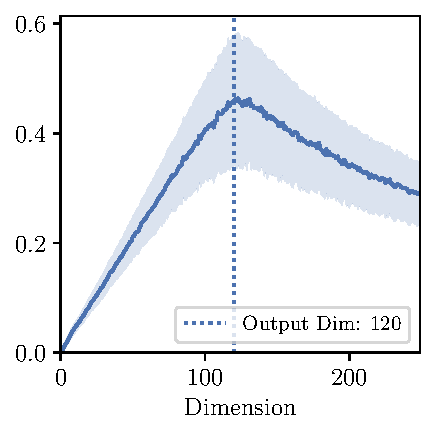
\includegraphics[width=0.49\textwidth]{Figures/SubspaceOverlap/NLeNet5_multi_hyperparam/DimOverlap_CIFAR10_LeNet5_normnew_fixlr0.001_X_LeNet5_normnew_fixlr0.01_X_LeNet5_normnew_fixlr0.01_momentum_fc1.pdf}
        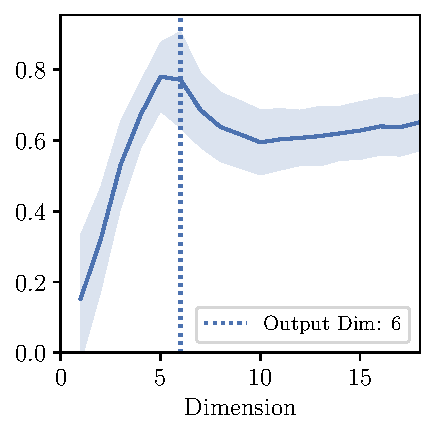
\includegraphics[width=0.49\textwidth]{Figures/SubspaceOverlap/NLeNet5_multi_hyperparam/DimOverlap_CIFAR10_LeNet5_normnew_fixlr0.001_X_LeNet5_normnew_fixlr0.01_X_LeNet5_normnew_fixlr0.01_momentum_conv1.pdf}
        \caption{Overlap between dominate eigenspace of layer-wise Hessian at different minima for fc1:LeNet5 (\textbf{left}) with output dimension 120 and conv1:LeNet5 (\textbf{right}) with output dimension 6.}
        \label{fig:intro_overlap}
    \end{subfigure}%
    \begin{subfigure}[b]{0.39\textwidth}
        \centering
        \captionsetup{justification=centering}
        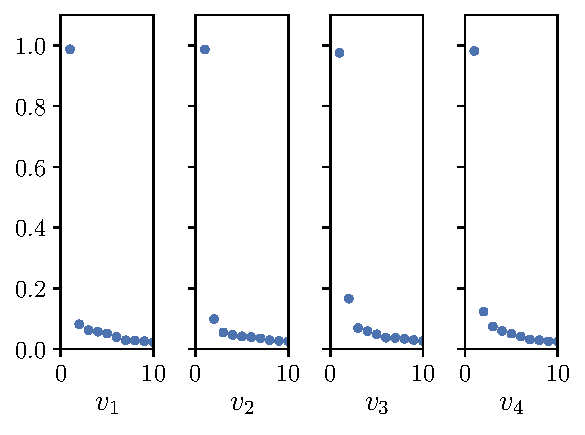
\includegraphics[width=\textwidth]{Figures/Eigenvec_single/Top_Eigenvector_sigs_CIFAR10_Exp1_LeNet5_fixlr0.01R1_E-1fc1.pdf}
        \caption{Top singular values of the top 4 eigenvectors of the layer-wise Hessian of fc1:LeNet5 after reshaped as matrix.}
        \label{fig:intro_lowrank}
    \end{subfigure}
    \caption{Some surprising observations on the structure of layer-wise Hessians.}
    \label{fig:intro_figs}
\end{figure}
\textbf{Structure of Hessians:} Consider two neural networks trained with different random initializations and potentially different hyper-parameters; their weights are usually nearly orthogonal. One might expect that the top eigenspace of their layer-wise Hessians are also very different. However, this is surprisingly false: the top eigenspace of the layer-wise Hessians have a very high overlap, and the overlap peaks at the dimension of the layer's output (see \cref{fig:intro_overlap}).
Another interesting phenomenon is that if we express the top eigenvectors of a layer-wise Hessian as a matrix with the same dimensions as the weight matrix, then the matrix is approximately rank 1. In \cref{fig:intro_lowrank} we show the singular values of several such reshaped eigenvectors. 

\textbf{Kronecker Factorization:} We show that both of these new properties of Hessians can be explained by a Kronecker Factorization approximation. Under a decoupling conjecture, we can approximate the layer-wise Hessian using the Kronecker product of the output Hessian and input auto-correlation. This Kronecker approximation directly implies that the eigenvectors of the layer-wise Hessian should be approximately rank 1 when viewed as a matrix. We also analyze the behavior of the two components: the auto-correlation of the input is often very close to a rank 1 matrix and the output Hessian often has around $c$ large eigenvectors. We show that when the input auto-correlation component is approximately rank 1, the layer-wise Hessians indeed have high overlap at the dimension of the layer's output, and the spectrum of the layer-wise Hessian is similar to the spectrum of the output Hessian. On the contrary, when the model is trained with batch normalization, the input auto-correlation matrix is much farther from rank 1 and the layer-wise Hessian often does not have the same low rank structure.

%\textbf{Leveraging Hessian Structure:}
%Better understanding of the Hessian can give more insights into optimization and generalization. 
As a direct application of our results, we show that the Hessian structure can be used to improve the PAC-Bayes bound computed in \citet{dziugaite2017computing}. %; we also show that the general structure of the Hessian suggests a simple way of incorporating second-order information in optimization without large overhead.

